% Chapter 4

\chapter{Implementation} % Main chapter title
\label{Chapter4} % For referencing the chapter elsewhere, use \ref{Chapter4} 

\lhead{Chapter 4. \emph{Implementation}} % This is for the header on each page - perhaps a shortened title

%----------------------------------------------------------------------------------------
In this chapter,Implementation using the approaches and tools that are considered to enable the Scalable Open Data Transformation as a Service, following the results from Chapter \ref{Chapter3} are discussed in detail. Firstly, the important high level general design aspects that are considered described with the reasons behind the decisions. Important design level and implementation level requirements, best practices and guidelines that we followed are explained with example implementation approaches.  Further, specific aspects that were considered according to the research motivation (The DataGraft project) are also notified. 
\section{Solution Design}
We detail the system architecture design and important components of architecture that will be detailed later, which enables the Scalable Open Data Preparation as a Service. First, we focus on the high-level components and architecture that compose them together to meet our requirements. We also describe the facts that we considered during our design phase that enabled our solution. 
\subsection{High Level Architecture}
The design of our scalable open data preparation tool follows Component Based Software Engineering (CBSE) \cite{CBSE} aspects, inherited from motivational project DataGraft. We aim to design according to \textit{separation of concerns}, and with the help of Service oriented Architecture (SOA) techniques the individual components will be integrated. This ensures that the solution components to be reusable and loosely coupled. 

Recalling our requirements from Section \ref{sec:fundamentals}, We want to provide a "\textit{Solution as a Service}" that is interactive, incrementally builds the data preparation with iterative transformations with near-real-time responsive results and execute the transformation on provided input data. Provided that we focus on providing a simplified solution that can engage with marginal audience without requiring technical skills, we require an \textit{automated system} that can  internally handle complex process activities. 

Our solution will be a web-based solution, to provide collaborative transformation, availability and accessibility and user friendly solution. It will be integrated to DataGraft project via its interactive tool Grafterizer. Making use of AJAX\footnote{https://en.wikipedia.org/wiki/Ajax\_(programming)} programming, we provide an interactive and responsive data preparation service. Our solution has 4 main components, which are mentioned below:
\begin{enumerate}
\item \textbf{Grafterizer} : The interactive tool of DataGraft, that can interactively build data preparation pipeline. Grafterizer is responsible to provide interactive user interface to build data cleaning and RDF mapping,  render data cleaning results in real-time and provide interface to execute a completed data preparation. Grafterizer closely follows  user interaction and perform data transformation and rendering seamlessly. It implicitly generates data transformation pipeline using a Domain Specific Language (DSL) and request the back-end to execute the transformation pipeline. 
\item \textbf{Mem-cache} : Mem-cache is an intelligent caching system, that caches the results for each step in transformation pipeline. Mem-cache optimizes the whole process by cleverly inspecting every transformation request with available cache and responds the cached result if a cache-hit is found, or delegates the request to back-end to execute the transformation and caches the new results for corresponding request. This can significantly improve the performance of the system, by eliminating redundant requests. 
\item \textbf{Scalable-graftwerk} : Scalable-graftwerk is a \textit{Data Transformation Engine as a Service}, that executes the transformation pipeline sent from client program \textit{on-the-fly}. This provides RESTFul \cite{restful} APIs to execute scalable open data transformation pipeline. This encapsulates the complex integration with scalable data preparation tool by wrapping the scalable transformation APIs with a DSL. The transformation pipelines generated and sent from client program are sent to Scalable-graftwerk using provided RESTFul APIs. Scalable-graftwerk's transformation execution engine executes the transformation pipeline sent with the request and replies the results as a HTTPResponse.  
\item \textbf{Sparker} : Sparker is the scalable open data transformation tool what will perform the actual job. Sparker comlies to the tools and requirements mentioned in Section \ref{sec:fundamentals} and Chapter \ref{Chapter3}. Sparker is wrapped using domain specific APIs by Scalable-graftwerk and exposed as a RESTFul service to users. 
\end{enumerate}
According to the discussions in Chapter \ref{Chapter3}, the solution should be scalable that can be scale-in or scale-out on a distributed environment. Figure \ref{fig:architecture} depicts how the components discussed above are composed together on cluster of distributed machines. 
\begin{center}
	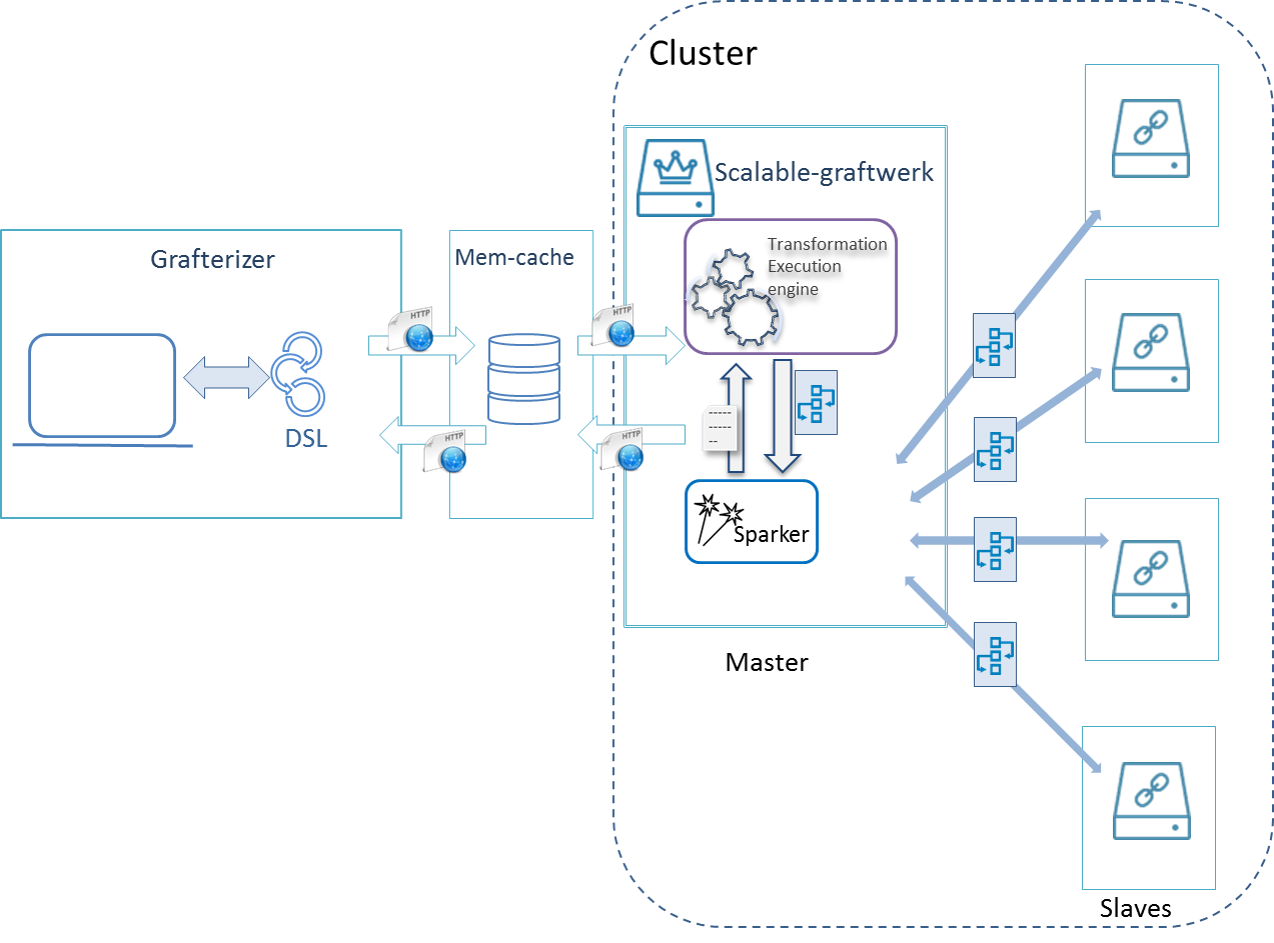
\includegraphics[width=38em]{./Figures/architecture}
	\begin{figure}[htbp]
    \caption{Scalable Data Transformation as a Service Architecture}
    \label{fig:architecture}
	\end{figure}
\end{center}
\subsection{Process Work-flow Diagram}
Figure \ref{fig:workflow} illustrates how a data preparation process is handled by our solution. User initially loads input file using Grafterizer. A user is given an option to decide whether to perform the interactive transformation on a sample of data or not. Open data can range from small to large volumes of data. Having said that, the option to create a sample allows user to decide according to the size of raw-data. 
\begin{center}
	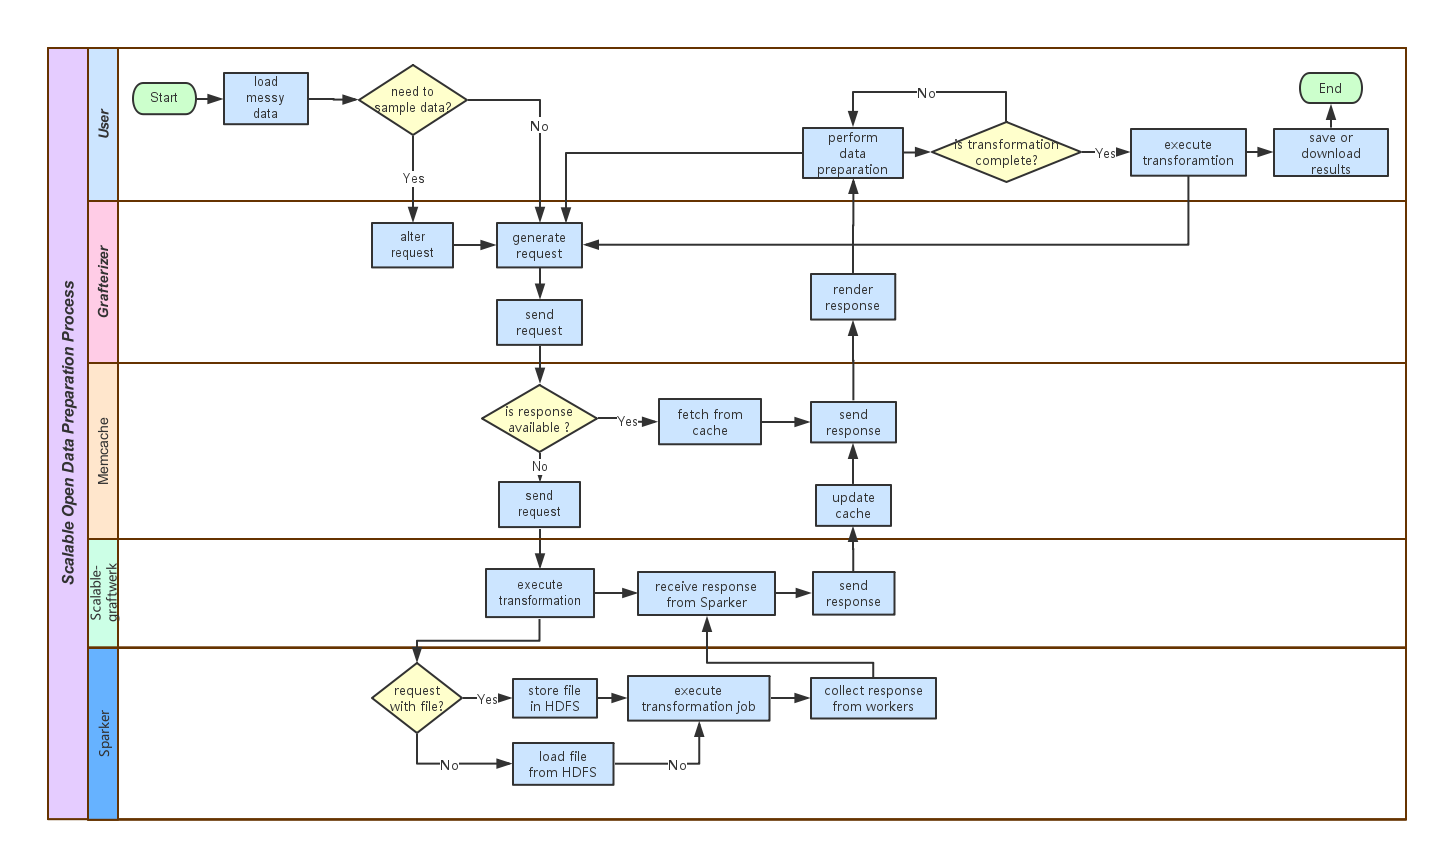
\includegraphics[width=55em, angle=90]{./Figures/work-flow}
	\begin{figure}[htbp]
    \caption{Optimized data preparation work-flow of large data}
    \label{fig:workflow}
	\end{figure}
\end{center}
If the data processed exceeds allocated quota of interactive transformation data size, it will be sampled by the system and initial file and sample files stored by back-end system. Then user can perform incremental, interactive transformation on data. When user is satisfied with transformation, user can execute the transformation on the whole data which is already stored at the back-end. Once the data transformation is performed, back-end will remove stale data.

\section{Solution components}
In this section we describe the basic components that are used to come up with the final solution engine, with supporting reasons for design decisions. 

\subsection{Sparker}
\label{sec:sparker}
The main challenge to be solved is to provide a scalable open data preparation solution using the techniques and technologies selected in Chapter \ref{Chapter4}. Provided that we follow \textit{separation of concerns}, we decided to implement the distributed open data preparation operations including data cleaning and linked data creation in a separate project called \textit{Sparker}. 
\subsubsection{Design level requirements}
\label{designreq}
We further analyzed the important requirement that need to be considered during our implementation and design level. Specifically, we require the data preparation tool to support,
\begin{enumerate}
\item Easily integrated with dynamic execution engine : The end-user solution is expected to be interactive and user friendly. This requires the data preparation operations to be built dynamically and executed on demand. Thus, it requires to provide Application Programming Interface (API) driven component.
\item Pattern oriented APIs : The data preparation operations are need to be provided as independent APIs that can be easily executed as pipeline of operations. To have intuitive pipeline creation of data preparation operations, all APIs should follow a pattern that can ensure seamless pipeline generation.
\begin{itemize}
\item \textit{\textbf{Chain-of-responsibility (COR) pattern}} : We need a pattern that can help to create pipeline of APIs provided. As we discussed earlier, data preparation will be performed iteratively and incrementally. Hence, the pipeline should reflect on incremental updates of data preparation.COR pattern a design pattern that has a parent command followed by series of processing commands. Each command has designated logic and input/output to handle and the rest are passed to the next processing command. This mechanism is also very helpful when adding an additional processing command at the end of the chain. The end result will contain the result of execution of all operations. 

For example if an API to select range of columns is given as take-columns(to,from) and drop-columns(to,from) to drop data, execution of take-columns(1,2) on data with columns A, B, C, D should result with a data with columns A, B, while if execution of drop-columns(1,2) then take-columns(1,2) should result in data with C, D, not with A,B or any other. 
\item Following the COR pattern and by adopting Builder pattern, we require the APIs to take same type of basic input parameter and should result in same type of output such that the pipeline can be easily created. 
\end{itemize}
\item Functional Separation between API : There should be clear separation between each API given, such that the execution of that operation does not provide results with side-effects at any of the combination of data preparation pipeline. Each API should be clearly broke down into specific behavior of the operation. (e.g. merging two columns should be separated from renaming merged column name). CBSE aspects can be considered during API level design too.
\end{enumerate}
\subsubsection{Functional requirements}
The next step is to identify the data preparation operations that need to be implemented. We gathered requirements from the motivational project and other related systems to provide a complete solution. Initially, we plan to implement data cleaning operations required by DataGraft and sample POC operation to create an RDF using simple mapping. However, we require the basic design should be able to evolve continuously according to future open data preparation needs. We conducted a feasibility analysis to see how can DataFrame APIs re-purposed to meet our needs. 
\subsubsection{Tools and Approaches}
An implicit requirement of our solution is to have a flexible low-level data abstraction that should be scalable such that it can be easily convertible to tabular data or to graph-based model. Referring to the systems in Section \ref{sec:relatedwork}, it can be clearly seen that the large-scale applications are focused on individual solution. One of the main impediment to evolve to fit open data requirements can be, lack of an interchangeable data abstraction. It is must our programming model and data abstraction meet this requirement. To confirm this requirement, we analyzed Spark's core components in detail. 
\begin{itemize}
\item \textbf{DataFrame} 

DataFrame is a collection of distributed data grouped into named columns (i.e. RDD with schema), that can perform relational operations on both RDD built from external sources and built-in collections \cite{SparkSQL}. DataFrame object can be easily created from RDD or from external resources as well as converted to RDD easily. It provides API for basic relational operations that can execute in parallel on distributed data.  Pipelines of operations can benefit from being lazily executed as mentioned in Section \ref{sec:spark}. Further, Figure \ref{fig:rdd-vs-dataframe} from an evaluation study from Databricks \cite{databricks-dataframe}(the designated paid maintainer of Spark), says that DataFrame is significantly faster than RDD when aggregation operations are performed.
\begin{center}
	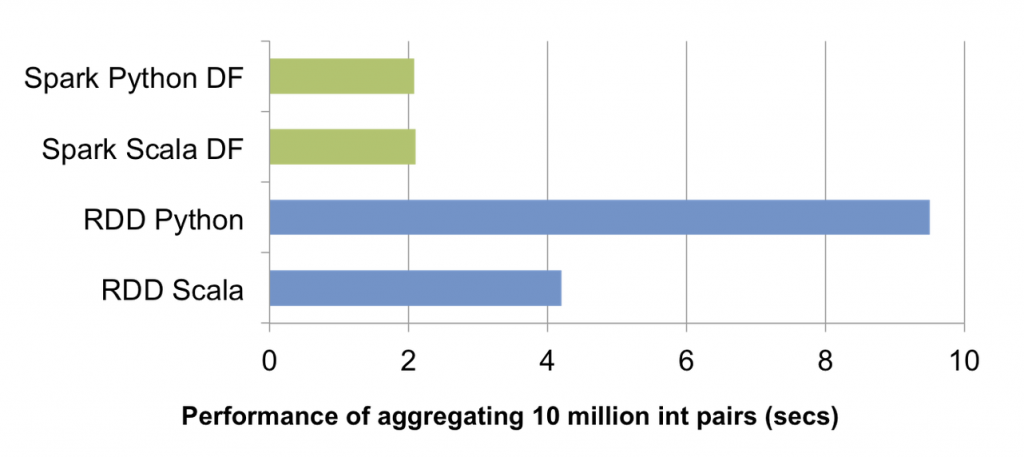
\includegraphics[width=38em]{./Figures/rdd-vs-dataframe}
	\begin{figure}[htbp]
    \caption{Programming components of Apache Spark Eco System \cite{databricks-dataframe} }
    \label{fig:rdd-vs-dataframe}
	\end{figure}
\end{center}
By utilizing lazy evaluation of ETL operations, Spark SQL can perform relational optimization \cite{SparkSQL} which satisfies our requirement (R6). Lastly, Spark SQL extends a novel optimizer called Catalyst. Catalyst supports both rule based and cost-based optimization \cite{SparkSQL}. This explains that DataFrame and Spark SQL can be exploited to represent messy data as tabular data and perform data cleaning, with internal relational optimization and query optimization.
\item \textbf{GraphX's Graph }

GraphX is a distributed graph computation model, that unifies graph-parallel and data-parallel computation \cite{GraphX}. This unified abstraction enables the same data to be represented as graph and tables without data movement or duplication. GraphX uses RDDs as the foundation for distributed collections and graphs. The property graph data model in GraphX was adopted from RDF graph \cite{RDFinGraphX}. The property graph corresponding to an RDF graph contains the predicates as edge properties and the subjects and objects as vertex properties. Thus, it is a strong base to create distributed graphs using RDD. 
\end{itemize}
Figure \ref{fig:dataabstraction} shows how the data abstractions discussed above can create an interchangeable data abstraction for our open data preparation system. The abstraction mentions the interchangeability of DataFrame to/from RDD and interchangeability of Graph to/from RDD. This can result in a flexible data abstraction that can solve our requirement.
\begin{center}
	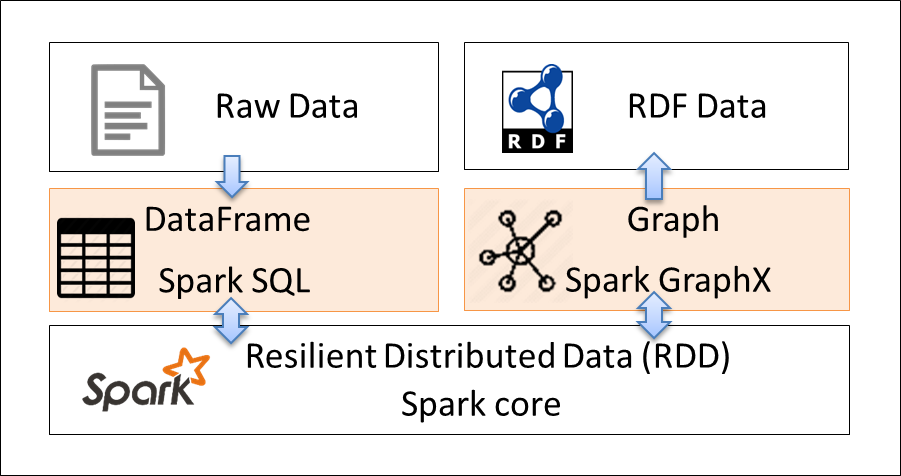
\includegraphics[width=35em, height=15em]{./Figures/data-abstraction-prog-model}
	\begin{figure}[htbp]
    \caption{Inter-changeable distributed data abstraction}
    \label{fig:dataabstraction}
	\end{figure}
\end{center}
Follwing the discussion in Section \ref{sec:sparker}, we designed our system as follows. Figure \ref{fig:package-diagram} shows the use case package diagram\footnote{http://agilemodeling.com/style/packageDiagram.htm} of Sparker. It shows that \textit{sparker.tabular} package, that is allocated to perform data cleaning activities on tabular data uses \textit{spark.sql} libraries including \textit{DataFrame} and \textit{sparker.rdf} package which is responsible for RDF creation uses  \textit{spark.graph} libraries to create graphs that uses \textit{Triplets}. Also there are internal supporting sub-packages named \textit{util} implemented to support data cleaning operations in DataGraft.
\begin{center}
	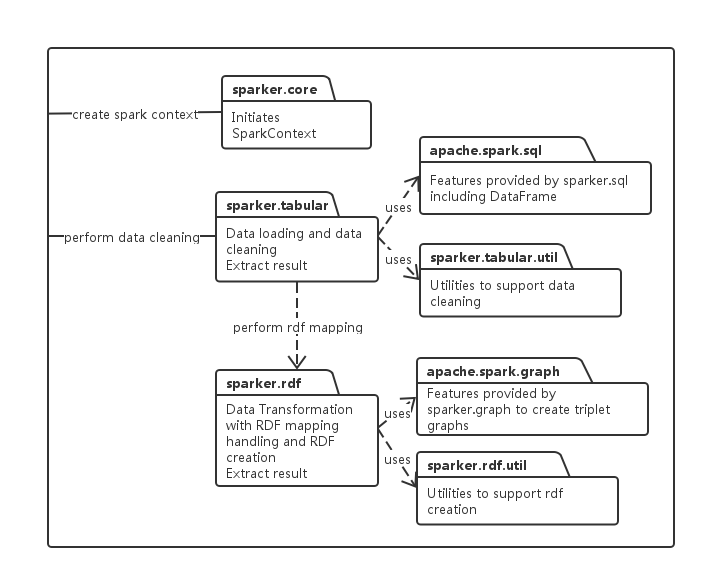
\includegraphics[width=35em, height=23em]{./Figures/Class_Diagram}
	\begin{figure}[htbp]
    \caption{Use case package diagram of Sparker}
    \label{fig:package-diagram}
	\end{figure}
\end{center}
\subsubsection{Choice of language and versions}
We decided to do the implementation using Scala\footnote{http://www.scala-lang.org/} among the languages Spark supports such as Scala, Python, Java and R. Scala is a current hype of Hybrid Languages that have insights of both Functional Programming (FP) and Object-Oriented-Programming (OOP) \cite{scala-book}. Scala runs on Java Virtual Machine (JVM) and interoperable with other JVM compatible programming languages. Hence, Sparker also can use any utilities implemented in JVM languages as well as can be used in all JVM languages. Moreover, Spark's initial implementations were using Scala, which ensures of strong and active community support and availability of feature implementations, extensions and plugins etc. We chose Scala 2.10.6 and Spark 1.6.0 versions for our implementation, as there were the latest stable releases. 
\subsubsection{Distributed data cleaning operations}
 The final challenge to solve in Sparker was to implement data preparations in distributed-data-parallel manner. We first focus on the implementation of data cleaning operations on tabular data. To make it clear, we introduce some basic explanations of how DataFrame behaves in distributed context and implementation on top of DataFrame should be approached. 
 
 \textbf{Spark and DataFrame Basics}
 
 Spark executes its tasks on RDD. Each RDD is split into number of partitions that may reside on different nodes of cluster. Number of partitions of RDD defines the basic level of distributed parallelism we can have. DataFrame extends RDD, which is also partitioned and located in different nodes of a cluster. Performing operations on a "distributed-table" is challenging. Following facts are important to be considered when data preparation functions are implemented.
\begin{itemize}
\item \textbf{Distribution of schema} : DataFrames are created with a schema that represents the structure of data, which is distributed to all partitions over distributed nodes. When the schema of the data is modified, the data need to be redistributed with updated schema, as all nodes should hold identical and up-to-date schema. When an operation is executed, every executor reads the schema and perform the operation based on the schema (if it depends on schema). 
\item \textbf{Distinction of transformations and actions of data cleaning operations} : Column level operations such as \textit{filter data, drop column} are easily performed on DataFrame, as they are usually types of \textit{transformations}. However, when \textit{actions} are performed on data (e.g. group and aggregate) then the driver needs to load the data from all partitions to a single memory and store them in external storage or re-partition the new RDD. Execution of \textit{actions} involve\textit{ data shuffling} from nodes, which is expensive than execution of \textit{transformation}. 
\item \textbf{Number of partitions} : As mentioned earlier number of partitions are the crutch of parallelization we can get during an execution. Ideally, Spark calculates the number of partitions according to the SparkContext and the data being processed. However, the DataFrame can be re-partitioned.  Having less number of partitions may result in less parallelism as well as having large number of partitions may result in huge overhead during data shuffling. 
\begin{itemize}
\item \textit{A Rule of Thumb} : A function should be always implemented with minimal data shuffling and auto-partitioning if the size data being process is subject to change, unless otherwise it is required. An implementation should try to consist more transformations or less frequent actions. 
\end{itemize}
\item \textbf{Memory allocation of Driver according the data being processed} : When data is shuffled from all nodes, the parent node should be able to hold the whole data in single memory without running out-of-memory problems. Hence, it is important to have a rough estimation of maximum size of data being processed and allocate Driver memory accordingly. 
\item \textbf{Addition of new data should be identically partitioned with primary data} :  Having said that, the RDD/DataFrame is partitioned, new data that need to added should also be identically partitioned. By \textit{identical} we mean equal number of partitions and equal number rows of each partition. The data that needs to be added should be partitioned in a way that it has one-to-one mapping to the rows that are in each partitions. 
\item \textbf{Rows that comply with schema} : Each row values of the table should comply with the schema, based on number of columns and structure of column and types of column.
\end{itemize}
Adhering to the above notes we implemented data cleaning functions on top of DataFrame API. 
\subsubsection{Implementation of Data Cleaning operations}
To explain how we carried out our implementation 1) adhering to the notes mentioned above, 2) utilizing the functional programming aspects 2) utilizing object-oriented programming aspects, we discuss few examples below. 
\begin{enumerate}
\item \textbf{Make dataset with a range of columns }

This operation doesn't involve in data shuffling as it is completely depend on columns that can be identically performed on all partitions. Using Scala APIs and DataFrame APIs we select a subset of column list using given range, perform a \textit{select} operation like \textit{SQL Select} to create new DataFrame. 
\begin{center}
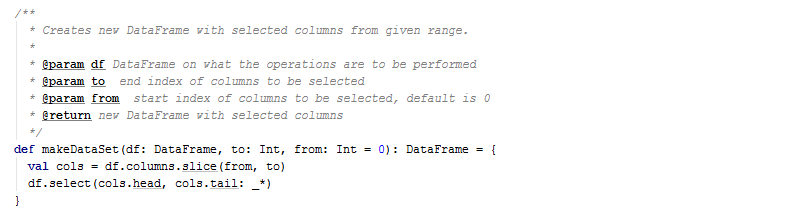
\includegraphics[width=38em]{./Figures/take-columns}
\begin{figure}[htbp]
\caption{Implementation of making dataset with range of columns}
\label{fig:take-columns}
\end{figure}
\end{center}
It can be clearly seen that the API provided is very intuitive and straight forward to use by the end user. 
\item \textbf{Merge columns}

When we want to merge a set of columns with a separator as shown in Figure \ref{fig:merge-columns-exp}, we need to create a new column i.e. it alters the schema. The below example explains how DataFrame API can be exploited when a new column is added. 
\begin{center}
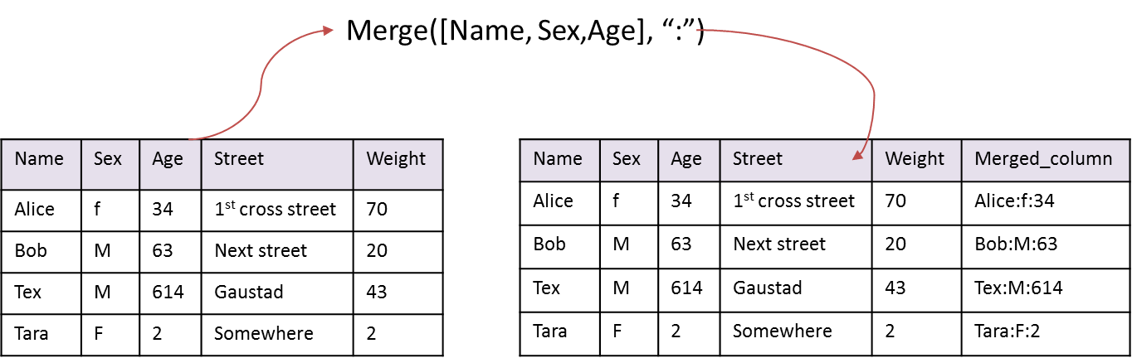
\includegraphics[width=30em]{./Figures/merge-col-exp}
\begin{figure}[htbp]
\caption{Explanation of merge columns}
\label{fig:merge-columns-exp}
\end{figure}
\end{center}
\begin{center}
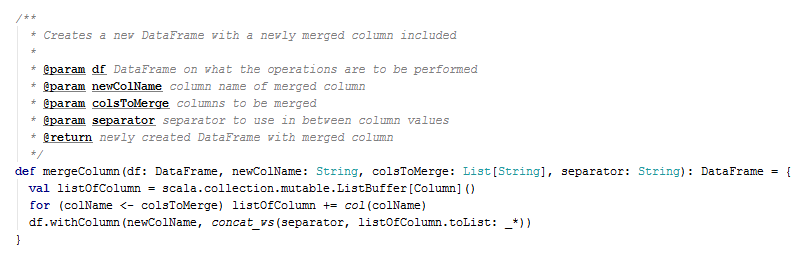
\includegraphics[width=38em]{./Figures/mergecolumn}
\begin{figure}[htbp]
\caption{Implementation of merging set of columns}
\label{fig:merge-columns}
\end{figure}
\end{center}
 The \textit{withColumn} API from DataFrame, handles the schema verification and if the column name provided is not available as a column already, it creates new schema with additional column with provided name (\textit{newColName}) and sends to all partitions. The \textit{concat-ws} is an implicit function provided by \textit{spark.sql} which takes arbitrary number of columns and merge them with provided separator. Every executor who sees the \textit{withColumn} function takes the \textit{newColName} from schema and sets the value from \textit{concat-ws} on right position. We must note that all these operations are performed based on columns, so data shuffle is performed. 
\item \textbf{Add row id }

When user wants to add a column with row id (row number), these row numbers nor a column to hold row numbers are part of the partitions already. This operation needs to change the schema as well as the partitions to add new data. Further the additional data need to be one-to-one mapped with existing partition data. As easy way to add incremental ids can be done by \textit{zipWithIndex} API provided by RDD.This operation creates the partitions of RDD with incremental index that is mapped to each row in every partition, preserving the order of rows.   
\begin{center}
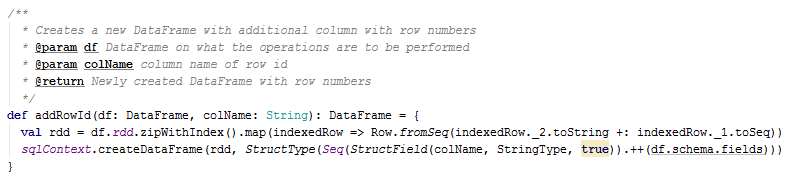
\includegraphics[width=38em]{./Figures/add-row-id}
\begin{figure}[htbp]
\caption{Implementation of adding a column with row id}
\label{fig:add-row-number}
\end{figure}
\end{center}
Making use of \textit{Map} operation, we create new Row with mapped index for each row. Then a new DataFrame is created using newly created RDD and newly created Schema which is called \textit{StructType} that has an additional column (\textit{StructField}).
This lets us to realize the level of technical and domain related abstraction provided by the implemented API.
\item \textbf{Melt data-set}

Reshaping\footnote{http://www.ats.ucla.edu/stat/stata/modules/reshapel.htm} data-set is an important requirement from data preparation sector. Reshaping data-set a powerful functionality that reshape the data according to user requirement. It is mostly categorized as \textit{wide-to-long} and \textit{long-to-wide}. We will see the implementation of a powerful reshape operation called \textit{\textbf{melt}}. Melt is a wide-to-long transpose operation of a data-set. 
\begin{center}
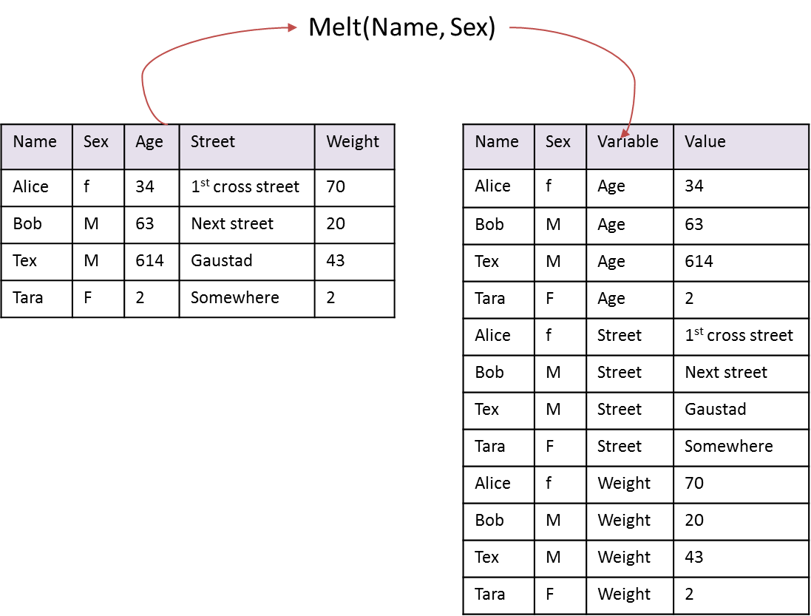
\includegraphics[width=30em]{./Figures/melt}
\begin{figure}[htbp]
\caption{Explanation of melt operation}
\label{fig:melt-exp}
\end{figure}
\end{center}
Melt operation is a very complex and expensive operation to perform. As reshaping data is not very common, we will first explain the behavior of \textit{melt} operation.Figure \ref{fig:melt-exp} depicts how a melt operation will result. Melt operation is performed to extract data that are included in column names. 
\begin{center}
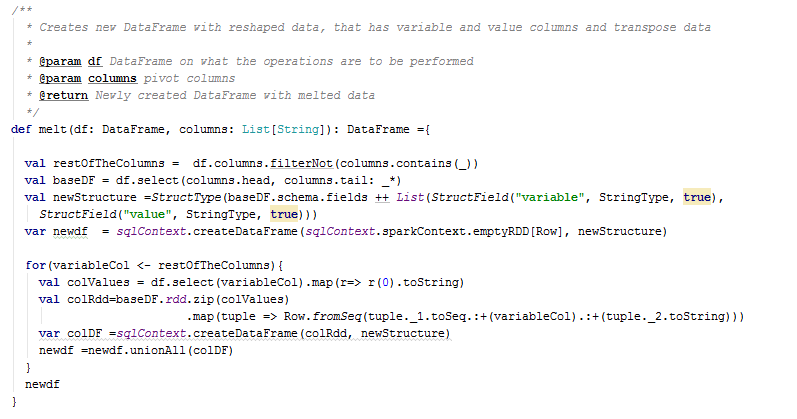
\includegraphics[width=38em]{./Figures/melt-impl}
\begin{figure}[htbp]
\caption{Implementation of melt operation}
\label{fig:melt-impl}
\end{figure}
\end{center}
To implement this functionality, we need to create new DataFrame with given pivot columns, create a schema with additional columns, then create \textit{Row}s for each columns with corresponding column name and value and perform a \textit{union} operation to merge these two DataFrames together, per column. 
\end{enumerate}
These examples illustrates that APIs eliminates the technical and domain related requirements a data-worker would need, and by providing simple, intuitive and schema-independent APIs that comply with the design requirements we discussed in Section \ref{designreq}. 
Table \ref{fig:features} shows the functions implemented by Sparker and brief description of the functions. 
\begin{center}
	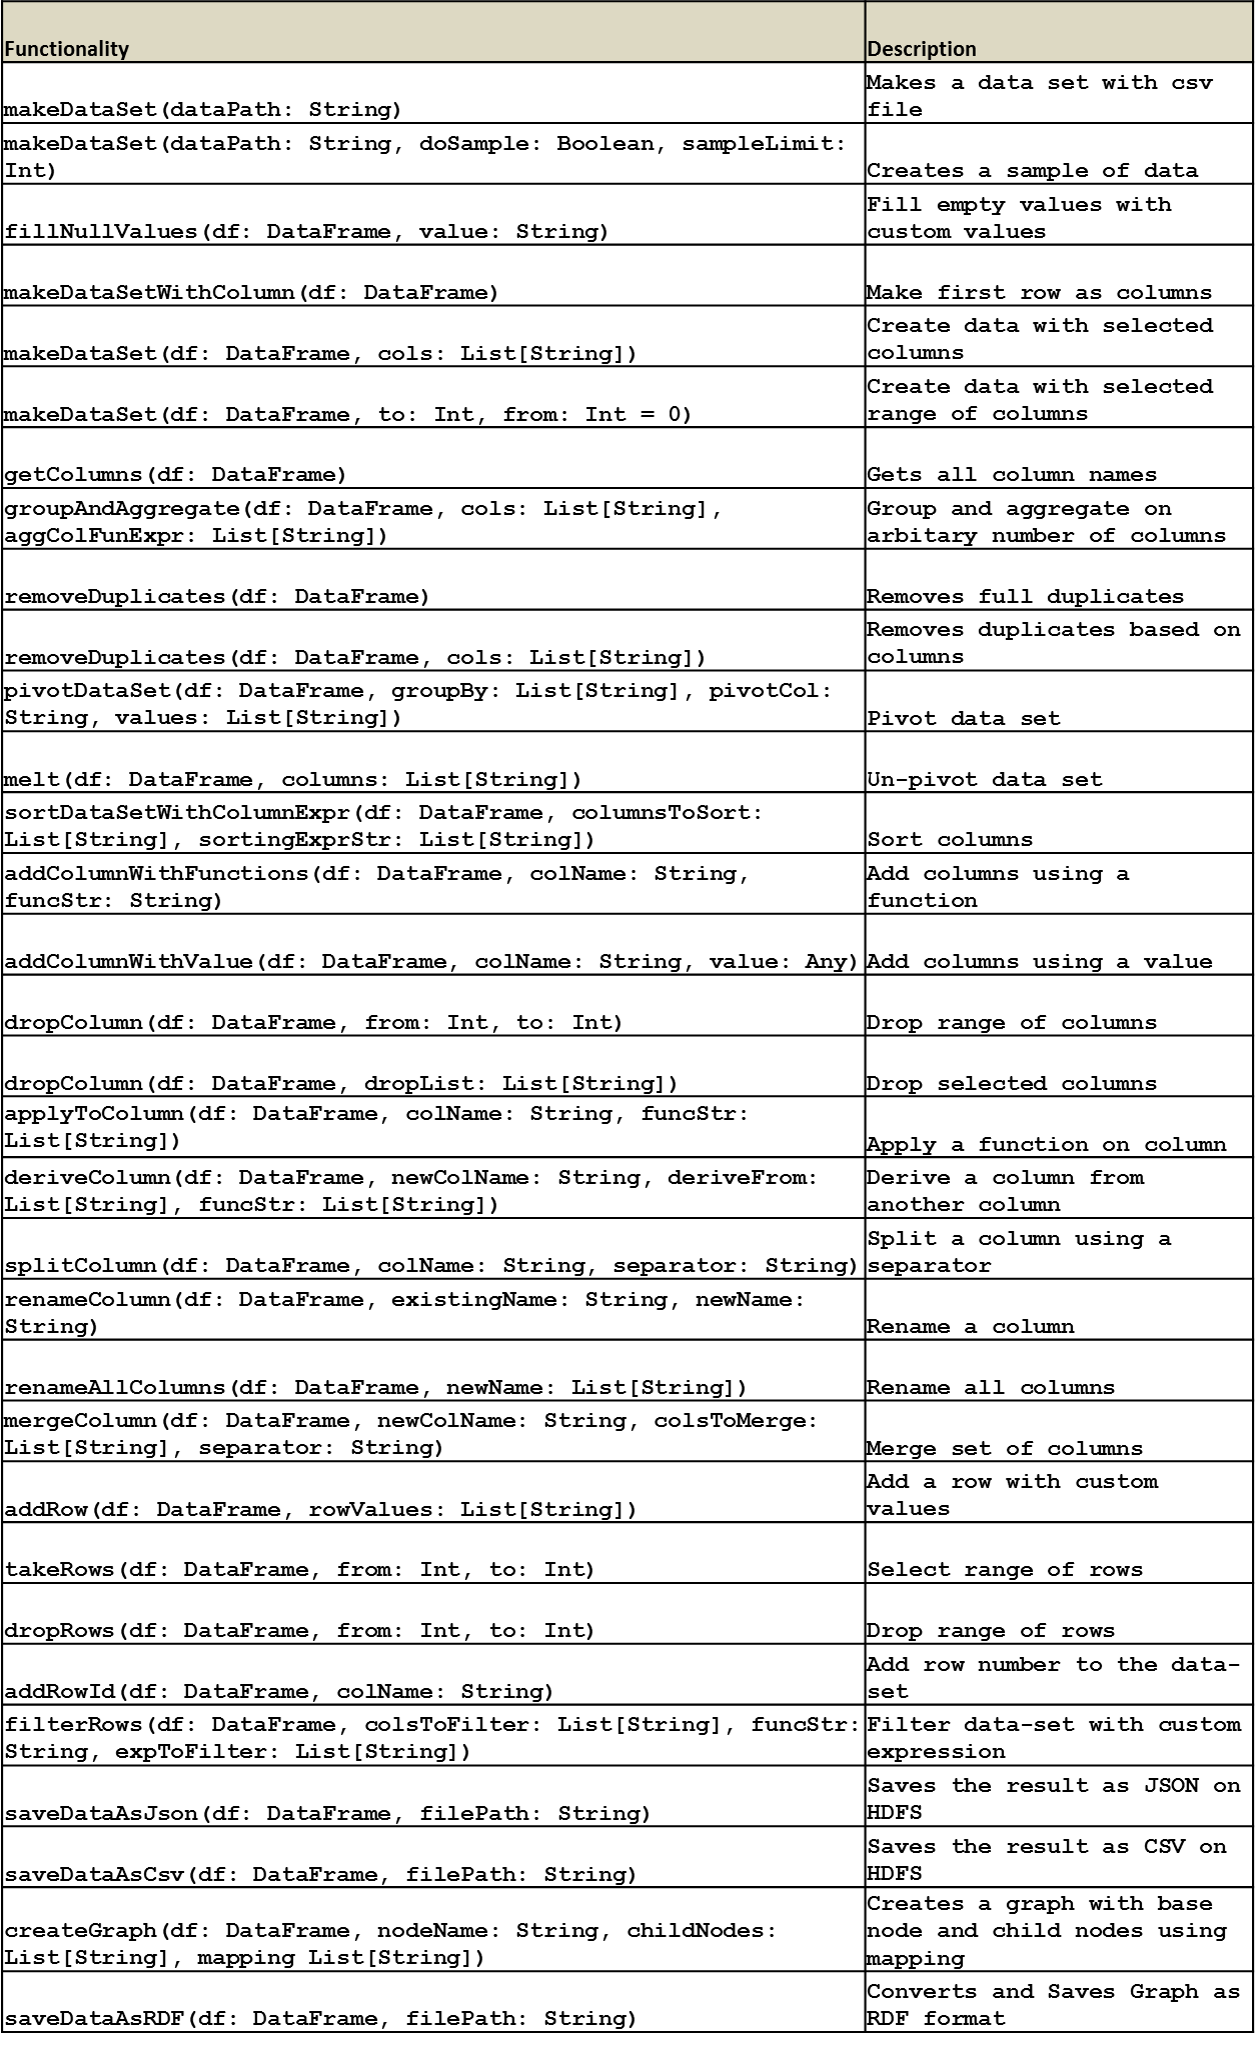
\includegraphics[width=35em]{./Figures/Picture2}
	\begin{table}[htbp]
    \caption{Table of Functions implemented in Sparker}
    \label{fig:features}
	\end{table}
\end{center}
\subsubsection{Implementation of RDF generation}
Generation of RDF from uncleaned data is our ultimate goal. RDF data of a tabular data can be generated by performing RDF mapping on tabular data. We can create a base node using a column or predefined literal. We currently, support simple RDF mappings, where a parent node is mapped with a child node using a property that explains the relationship between them. This results in specifying two columns of table and mapping information for each mapping ( e.g. Column "personID" can be mapped to column "name" with a mapping of foaf:name, i.e name property from foaf (Friend of a friend) vocabulary).  We create vertices of both specified columns, which contains unique VertexID as required by Spark graph for each row. Then we create an Edge that has (parentVertexId, childVertexId, mapping) for each record for each record. This results in a graph of \textit{Triplets}. Likewise, we perform this two operations for each mapping specified in a graph. Once the mapping is finalized,  we generate RDF in the form of N-triple, by concatenating values in each triplet of given graph. 

\subsection{Scalable-graftwerk}
Scalable-graftwerk is a service that provides dynamic transformation execution engine that executes a DSL and also provides an adapter of Sparker. We will discuss, the important features provided by Scalable-graftwerk and how it enables our solution to be interactive.
\subsubsection{Functional requirements}
\label{engine-req}
The important requirements to solve in Scalable-graftwerk are :
\begin{itemize}
\item \textbf{An environment with a dynamic language} : Data cleaning transformations are interactively created from client side. They should be built using a dynamically typed language also called as \textit{dynamic language }. A dynamic language is a programming language that just not gets compiled and run, but also can be added, changed functions at run-time and evaluated at run-time). 
\item \textbf{Dynamic execution engine of transformation} :  Each stage in a transformation pipeline should be evaluated dynamically during the interaction. Transformation pipelines are essentially programs or meta-data that needs to be dynamically executed. An execution engine should be created to evaluate the generated pipeline on-the-fly to provide response immediately.
\item \textbf{Dynamic APIs that wraps open data preparation functions} : Provided that we have an execution engine that can execute programs of a dynamically typed language, since we are using Sparker for scalable open data preparation, those data preparation features mentioned in Figure \ref{fig:features} must be adapted using the selected dynamic language, such that it can be used to create  transformation pipeline and executed by execution engine.
\item \textbf{RESTFul APIs} :  Lastly, our goal is to provide Scalable open data transformations as a Service. The requirements discussed above should be exposed as Web Service APIs that can be integrated with external systems. We chose to use RESTFul APIs adhering to the system designs of DataGraft. 
\end{itemize}
\subsubsection{Tools and Approaches}

\textbf{Clojure}

Referring to above requirements, we need a dynamic language to perform interactive execution of transformation pipelines. We used Clojure \cite{clojure} a functional programming language and a dialect of LISP\cite{lisp} programming language (a dynamic high-level-language). Clojure inherits  and \textit{dynamic typing} and fully \textit{parenthesized prefix notation} (i.e. a programming logic is mentioned using parenthesis having a function to evaluate and related parameters within the parenthesis e.g. \textit{\textbf{(add 1 2)}}) from LISP. Clojure runs on JVM and supports concurrent programming. Specially, Clojure provides \textit{\textbf{macros}}, which is a language construct in Clojure that can easily extend the language at compile time. Since Clojure is a dynamic language, type annotations are not required for code to run. Moreover, Taking advantage of  interoperability of JVM languages, Clojure can be easily integrated with other JVM languages. Since Clojure is a dynamically typed language that can run on JVM whereas Sparker is implemented using Scala which is also another JVM based language, the choice of Clojure fits our context well, than other dynamic languages such as Ruby, PHP, Lua and Perl. 

\textbf{Ring Server and Compojure Routes}

To provide a RESTFul service, We need a web server (A computer system that can process requests via Hypertext Transfer Protocol (HTTP), the basic network protocol used on the World Wide Web) that can process Web Services. We implemented our RESTFul Web Services using open sourced libraries including Ring\footnote{https://github.com/ring-clojure/ring} and Compojure\footnote{https://github.com/weavejester/compojure}. Ring is a Clojure library that provides abstractions of HTTP into simple and unified APIs. Ring allows a web application to be a collection of small independent modules. Routes in Ring are small modules that can compose a Ring Application. Compojure is a routing library for Ring, which provided simple APIs as macros\footnote{http://clojure.org/reference/macros}, that can be simply implemented as RESTFul Services. We chose Ring and Compojure as there were the state-of-the-art implementations of our requirements and widely used by Clojure community. 
\subsubsection{Sparker's Adapter in Clojure}
We need a \textit{dynamically typed} version of Sparker's functions. Following \textit{adapter design pattern} , we implemented an adapter that wraps Sparker's functions implemented as Scala APIs into equivalent Clojure functions. 
\begin{center}
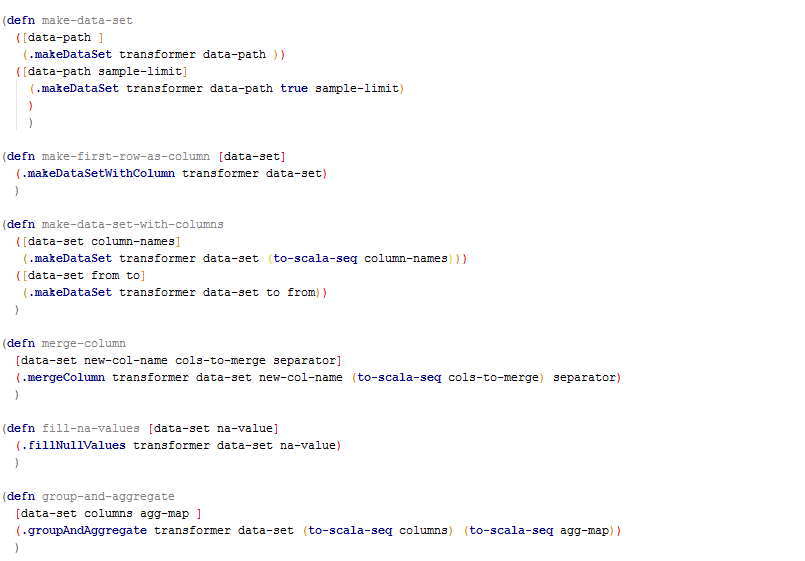
\includegraphics[width=36em]{./Figures/wrapper}
\begin{figure}[htbp]
\caption{Part of Sparker's adapter in Clojure}
\label{fig:wrapper}
\end{figure}
\end{center}
Figure \ref{fig:wrapper} shows the adapter of Sparker's functions in Clojure. A sample data transformation pipeline is shown in Figure \ref{fig:sample-pipeline} that creates a data-set with columns from first-row, then selects columns ranging from 0 to 15 and, then select specific columns by column names and lastly removes duplicates in groups based on provided set of columns. This example proves that the design requirements considered in Section \ref{designreq} have resulted in simple and easy creation of transformation pipeline. 
\begin{center}
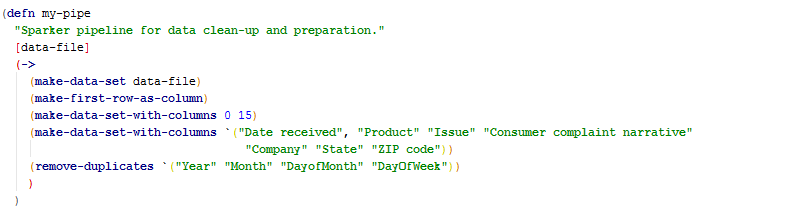
\includegraphics[width=36em]{./Figures/sample-pipeline}
\begin{figure}[htbp]
\caption{Sample pipeline using DSL of Scalable-graftwerk}
\label{fig:sample-pipeline}
\end{figure}
\end{center}
Clojure's thread first macro\footnote{https://yobriefca.se/blog/2014/05/19/the-weird-and-wonderful-characters-of-clojure/} take an initial value and thread this value through a number of forms. By passing output from previous command to following command this ensures that data pipeline processed for given input. 
\subsubsection{Scalable Data Transformation as a Service}
We adopted an open sourced implementation called Graftwerk\footnote{https://github.com/Swirrl/graftwerk}, which can perform similar tasks mentioned in Section \ref{engine-req}. Graftwerk has an in-built sandbox which securely execute arbitrary Clojure codes. Sandboxes are created with a secured execution context and can be configured to avoid execution of codes with security threads. Even though having a sandbox in a dynamic execution engine provides security, such sandbox with restricted context prevented us from executing Spark related code. Thus, we implemented an execution engine using Clojure's core library that can execute only the DSL defined in Scalable-graftwerk. Scalable-graftwerk's dynamic execution engine and scalable data transformation features can be accessed by external systems using provided RESTFul API.  Those Web Service APIs provided by Scalable-graftwerk eliminates execution and integration complexity of Sparker functions. 
Sample API implementation using routes and how such API can be used using a RESTFul client is shown in Figure \ref{fig:sample-route} 
\begin{center}
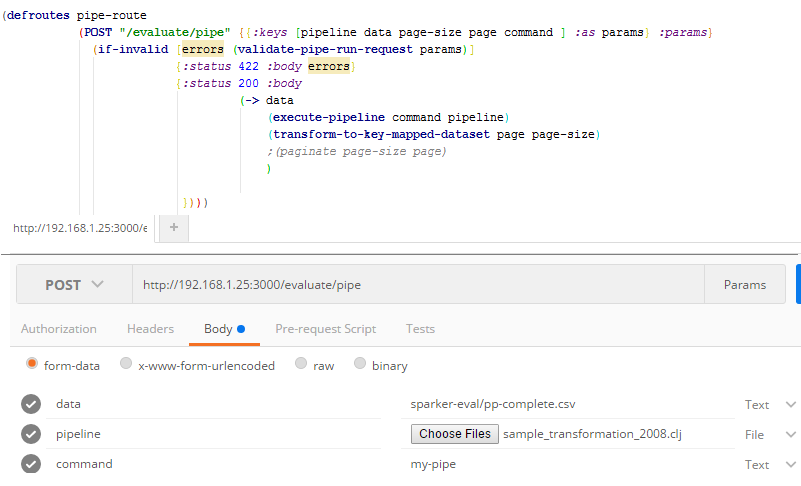
\includegraphics[width=36em]{./Figures/sample-route}
\begin{figure}[htbp]
\caption{RESTFul API of transformation engine and Execution of a sample transformation}
\label{fig:sample-route}
\end{figure}
\end{center}
\subsection{Grafterizer}
Grafterizer is the the interactive data transformation tool of DataGraft. Grafterizer has user friendly, spreadsheet like interface to display tabular data and user interfaces that provide easy means to build transformation pipeline. Once the data is cleaned, user can create RDF mapping using Grafterizer's RDF Mapping interface. During the data preparation process, Grafterizer automatically builds corresponding transformation pipeline scripts, creates and sends HTTPRequest to given RESTFul APIs. Once the response is received, using the response headers Grafterizer renders data in tabular format. 

\subsubsection{Functional requirements}
Grafterizer has a code generator, that can generate transformation pipeline code according to user's input. We need to adapt this code generator to build Scalable-graftwerk's DSL scripts for each data preparation process according to user input. Generated 

\subsubsection{Tools and Approaches}
Since we reused existing implementation of Grafterizer, we had to adapt some of the existing modules to create Scalable-graftwerk's DSL compatible code. In this section, the approaches we followed to automatically generate required transformation pipeline scripts in Scalable-graftwerk's DSL. 

\textbf{AngularJS}

Grafterizer is built using AngularJS, an open source web application framework, aims to provide simplified development and testing of web applications by providing model-view-controller(MVC) and model-view-view-model (MVVM) architectures, built in JavaScript and TypeScript. jsedn\footnote{https://github.com/shaunxcode/jsedn} is a JavaScript implementation of EDN. jsedn helps to create EDN formats from JavaScript. Using jsedn we create Scalable-graftwerk's DSL scripts which is on Clojure for each transformation pipeline command. 

\textbf{Extensible data notation and jsedn library}

Extensible data notation\footnote{https://github.com/edn-format/edn} (EDN) is a subset of Clojure. EDN is also used as data transfer format like JavaScript Object Notation(JSON). EDN supports rich set of data notations and covers basic set of data structures common to most programming language. Simple Clojure programs can be represented by EDN format. EDN notations helps to represent basic data structures easily. For example a list of 1, 2, 3 can be mentioned as (1 2 3) whereas a vector of 1, 2, 3 can be mentioned as [1 2 3], Strings can be enclosed in double quotes and keywords are prefixed with : like :id. Such simplified notation helps to create EDN format from basic structures easily. 

\subsubsection{Code generator and pipeline builder}
As mentioned earlier, we used \textit{jsedn} to notate Scalable-graftwerk's DSL for each transformation pipeline. EDN also doesn't need type-annotations of data being represented like Clojure. This eliminates the complexity of mentioning types and classes of objects like other programming languages. A Clojure function is a list of command and parameters. Hence, creating an EDN list will result in a Clojure function. Symbols in EDN are used to represent identifiers. A function is represented as \textit{Symbol} in Clojure. Creating a symbol using EDN inside a list will result in a Clojure command. 
\begin{center}
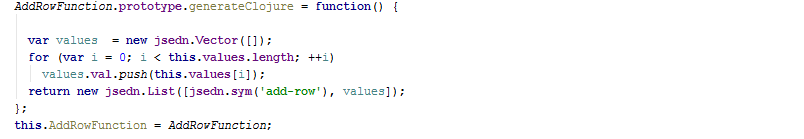
\includegraphics[width=36em]{./Figures/generate-clojure}
\begin{figure}[htbp]
\caption{Sample code generation of DSL from Grafterizer}
\label{fig:sample-jsedn}
\end{figure}
\end{center}
A sample generation of DSL from Grafterizer is shown in Figure \ref{fig:sample-jsedn}. We create a list that contains a symbol that represents a command followed by the input parameters to corresponding command. In this example the values that will be used to create a new row are passed as input parameters in a vector. Those values are derived from user interface using AngularJS. 




